\chapter{Vanliga fel i notsättning}
\begin{centering}
\textbf{ur \textit{Stilguide för orkesterarrangemang} av \\ Markus Silberstein Hont, maestro, Kårspexet 2013}

\textit{med revideringar, kommentarer och förtydliganden av \\ Axel Stenberg, kapellmästare, Kårspexet 25/26}

\vspace{1em}
\end{centering}

\section{Inledning}
Ett sångnummers partitur och dess stämmor ska liknas vid ett scenmanus för orkestermusiker. På samma sätt som en illa formulerad text kan förstöra en annars väl genomtänkt historia i en film kan ett vackert och kreativt arrangemang förstöras av att partituret är dåligt skrivet eller att layouten är ologisk. Man ska inte underskatta den psykologiska skillnaden mellan att spela samma arr i en svår respektive lättläslig version. ''Det låter aldrig bättre än det ser ut'', som någon stel moralist en gång valde att uttrycka det, är faktiskt ett väldigt bra rättesnöre när man tydligt vill förmedla sina storslagna musikaliska idéer till en orkester. 

Att göra en effektiv layout till sitt arr behöver inte vara svårare än att man följer en samling enkla regler som är konventionella i	professionella sammanhang världen över. Viktigt att komma ihåg är dock att \textit{snygga layouter tar tid att göra}. Men det är alltid mödan värt och man minskar risken för att behöva få tillbaka sitt (kanske oläsliga) arr av sin beställare för att snygga till utseendet. Nedan följer de, i min mening, viktigaste sakerna att tänka på när man formaterar sitt partitur. Första avsnittet handlar om notation, det andra om layout.

\newpage
\section{Swing, shuffle eller rakt?}
Ett vanligt sätt att göra ett arr mer svårläsligt är att försöka notera låten i ett annat rytmmönster än det som låten passar bäst i. Det finns tre huvudsakliga mönster, och de skiljer sig från varandra endast i hur åttondelarna spelas: raka, swing- och shuffleåttondelar.

Raka åttondelar är de vanligast förekommande och de spelas med jämna (tids-)avstånd mellan varandra.

Swing är vanligast inom jazz men går lätt att hitta i många andra genrer. Många klassiska musikalnummer är skrivna i swingtempo. I praktiken låter swingåttondelar som åttondelstrioler där den mittersta tonen är tyst:

\begin{center}
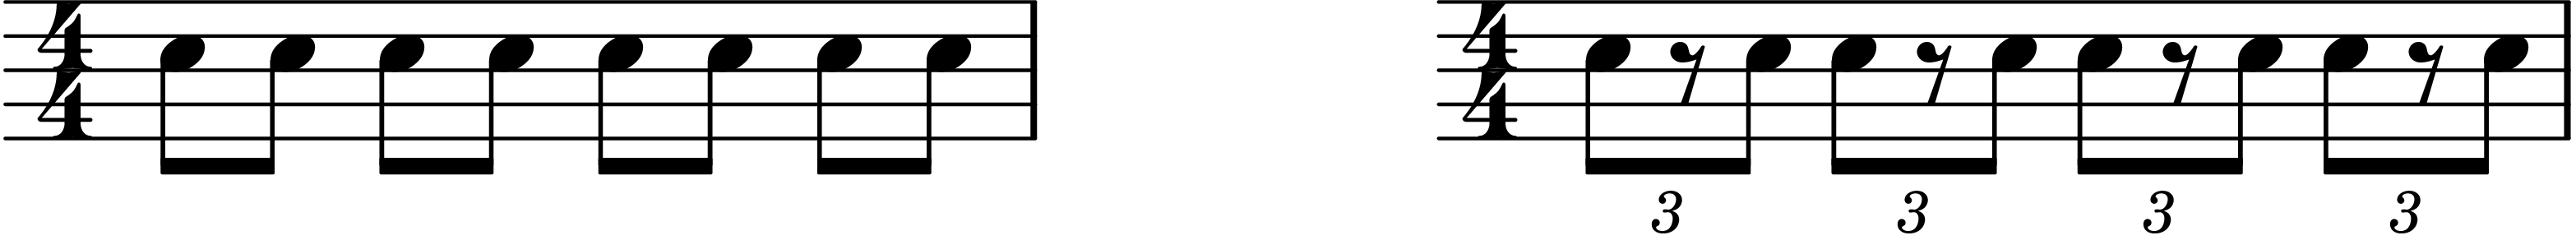
\includegraphics{lilypond/swing.cropped.png}
\end{center}

För att inte förvirra instrumentalisterna måste man indikera att man vill att stycket ska spelas med den här typen av åttondelar. Det görs längst upp på sidan, antingen genom att skriva ”swing” eller genom att inkludera följande figur: 

%\begin{center}
%    \includegraphics[width=0.2\textwidth]{lilypond/swing-mark.cropped.png}
%\end{center}

En shuffle är väldigt likt ett swingstycke, eftersom de bygger på samma triolkänsla. Men skillnaderna är framför allt två. En takt i swing betonar tydligt det andra och fjärde slaget medan en shuffletakt har en mycket jämnare betoning på varje fjärdedel. Så långt ingen skillnad i hur de noteras rent tekniskt. Men i shufflelåtar spelar man, till skillnad från i swinglåtar, ofta figurer med hela trioler och alltså inte triolfigurer där den mittersta triolåttondelen utelämnats.

När man skriver en shuffle måste man bestämma sig för om man vill notera i 12/8 eller i 4/4. Fördelen med 12/8 är att man slipper skriva ut triolbågar över åttondelarna, vilket man måste göra i 4/4. En nackdel med 12/8 är att många amatörmusiker är något ovana vid taktarten, och ser därför hellre 4/4. I övrigt är det upp till arraren att välja. Figuren nedan visar två ekvivalenta takter skrivna på var sitt sätt. Lägg märke till hur noterna är grupperade i 12/8-takten för att tydliggöra att det är fyra huvudmarkeringar per takt. 

\begin{center}
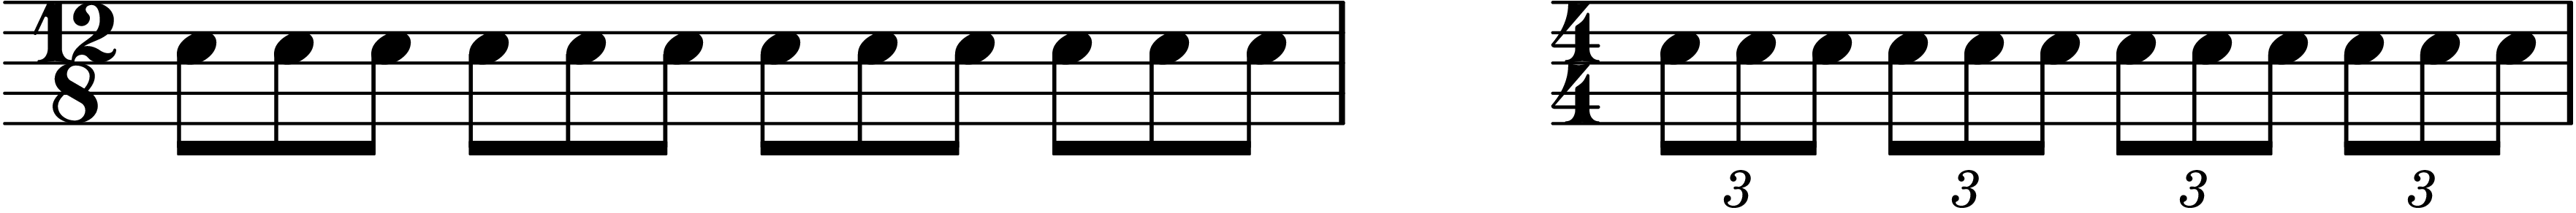
\includegraphics{lilypond/shuffle.cropped.png}
\end{center}

\newpage
\section{Gruppering av noter}
Det finns många sätt att skriva en och samma rytm i en takt. Men det finns flera sätt som gör rytmen svår att känna och därmed även svår att spela. Ett vanligt misstag som många gör är att skriva rytmen helt frikopplad från taktartens puls. Nedan finns en och samma takt skriven på tre olika sätt:


\begin{center}
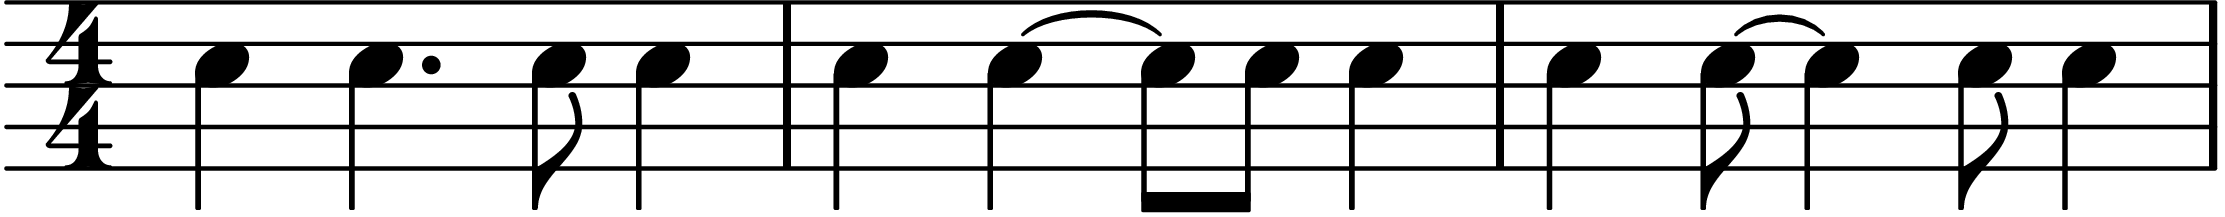
\includegraphics{lilypond/grouping.cropped.png}
\end{center}

Det är dock bara den mittersta takten som är korrekt skriven. Varför? Därför att de övriga två är frikopplade från pulsen. Taktarten 4/4 har två starka taktslag, det första och det tredje; Det andra och fjärde betraktas som svaga taktslag. De två felaktiga skrivsätten döljer det andra starka taktslaget genom att låta en not överlappa det. Den korrekta takten är skriven så att man kan se det tredje taktslaget, vilket man måste kunna göra för att förankra rytmen vid pulsen.

Det sistnämnda är en mycket viktig regel: \textbf{I en 4/4-takt måste det tredje taktslaget vara synligt.} Liknande regler gäller för andra taktarter, men där råder inte lika stark konsensus. Det som styr är hur man vill att melodin ska vara grupperad inom takten. En 5/4‐takt kan till exempel delas upp som 3/4 + 2/4 såväl som 2/4 + 3/4, bland annat. I dessa fall måste det fjärde respektive det tredje slaget vara synligt. (Om åttondelarna i 12/8‐takten här ovan hade varit grupperade i par så hade det implicerat att den bör spelas i vals-känsla istället för i 4/4‐takt som dess nuvarande grupper om tre talar om.)

En annan vanlig svårläslighet som ovana arrare gärna använder är överdrivet många bindebågar. Nedan finns exempel på två vanliga misstag:

\begin{center}
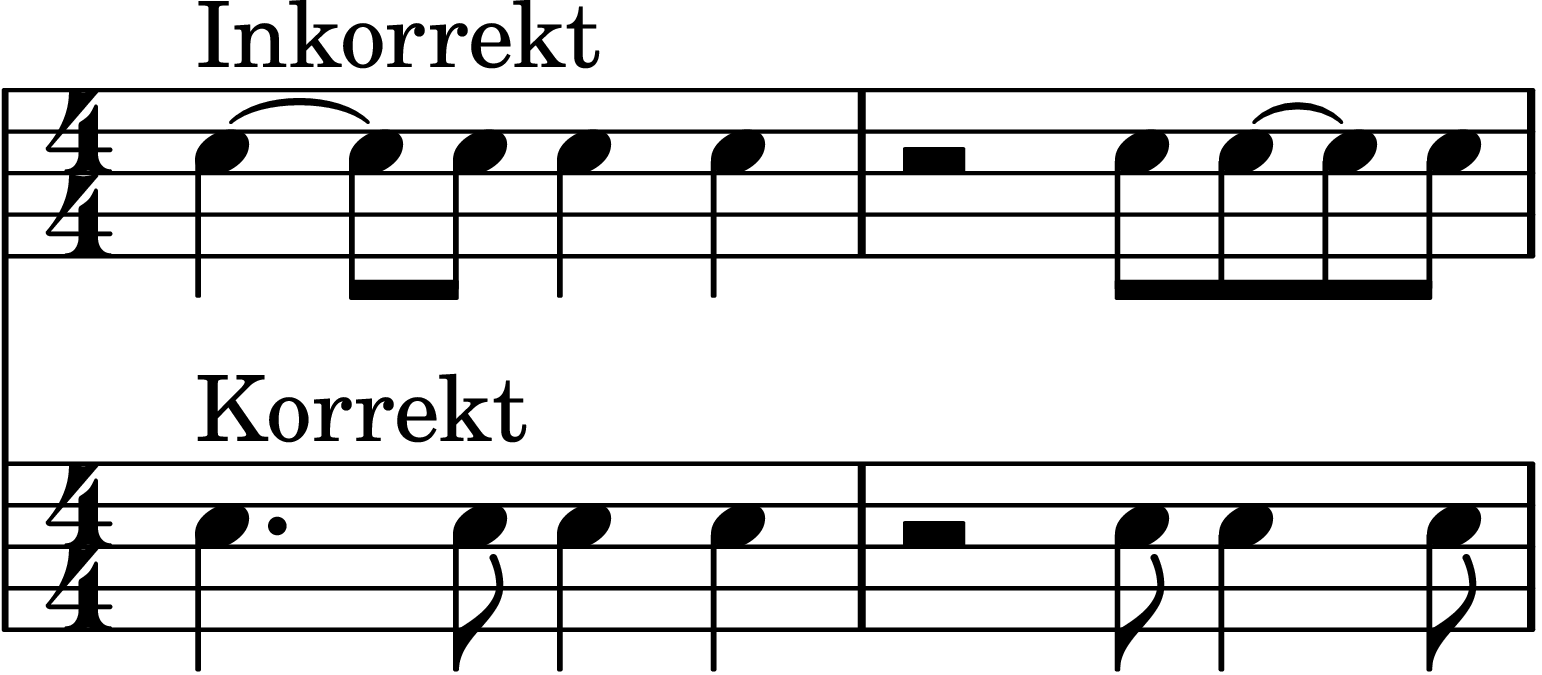
\includegraphics{lilypond/ties.cropped.png}
\end{center}

Att skriva noter så koncist som möjligt är ofta ett bra ledmotiv (så länge regeln med det synliga tredje taktslaget följs).

\vspace{2em}
\noindent\fbox{%
    \parbox{\textwidth}{%
        \textbf{Musescore}

        I Musescore finns ett verktyg för att automatiskt gruppera noter enligt på det sätt som beskrivs ovan. Verktyget heter \textit{Regroup rhythms} och finns i kategorin \textit{Tools} i menyraden. På svenska heter samma verktyg \textit{Återställ rytmgrupperingar} och finns i kategorin \textit{Verktyg}. Markera de takter som ska rättas till innan du startar verktyget, eller avmarkera taktmarkeringen för att korrigera alla takter i stycket.
    }%
}

\newpage
\section{Dynamik, accenter och text}
Det finns många bra verktyg för att förmedla hur man vill att instrumentalisterna ska spela tonerna och rytmerna på ens eget sätt. Tre av de viktigaste är dynamik, accenter och text.

\vspace{1em}
\textbf{Dynamik} är viktigt för att göra låten levande så att lyssnaren inte tappar intresset halvvägs igenom. Hur dynamiken används rent musikaliskt är förstås helt och hållet upp till arraren, men det finns framförallt två viktiga saker att komma ihåg. För det första så beror tolkningen av dynamikmarkeringarna mycket på sammanhanget och på vem som dirigerar orkestern – ett mezzo forte kan låta olika starkt från fall till fall. Något som man däremot alltid bör kunna lita på är att alla markeringar inom ett arr förhåller sig lika till varandra relativt sett. För det andra måste man tänka på att alla instrument inte kan spela alla dynamikmarkeringar i alla register. Det är till exempel väldigt svårt för ett träblåsinstrument att spela väldigt ljusa toner väldigt tyst.

\vspace{2em}
\noindent\fbox{%
    \parbox{\textwidth}{%
        Något annat viktigt att tänka på är att dynamik-markeringar i första hand är till för orkestern, och i andra hand för att få Musescore-filen att låta bra. Detta gäller självklart alla aspekter av notationen, men det är främst i dynamiken som man lätt glömmer det. Skriver man mezzo-forte i alla stämmor kommer orkestern att (till sin bästa förmåga) låta dynamiskt balanserat. I praktiken betyder det kanske att trombonerna tar i lite mindre än fiolerna, men det är precis vad mezzo-forte betyder. Musescore har däremot ingen uppfattning om den totala ljudbilden, utan varje instrument spelar starkare eller svagare enbart utifrån sin egen dynamik. Om något instrument verkar alldeles för svagt eller för starkt är lösningen istället att justera volymen i mixer-vyn. 

        \textbf{Ett exempel:} En glad och nöjd kårspexarrare lämnar in sitt arr. Klarinett-ljudet i Musescore var för lågt i sektionen där alla spelar mezzo-piano, så vår lösningsorienterade arrare sätter dit ett forte för att åtgärda problemet. Väl på repet sänker resten av orkestern volymen så mycket de kan, och vår stackars klarinettist blåser sig röd i ansiktet för att lyckas hålla ett forte-solo över resten av orkestern. Längre fram spelar alla forte, men trumpeten blev \textit{för} högljudd, och byttes till ett mezzo-piano. Trumpetaren sitter sedan på repet och känner sig lite överflödig, för hen hörs ju ändå inte. Detta var inte alls vad arrangören hade tänkt sig, men det var så det blev skrivet. 
    }%
}

\vspace{1em}


\textbf{Accenter} är små nyanser som kan läggas till de enskilda noterna. De kan ofta ersätta användandet av onödigt många pauser och/eller dynamikmarkeringar. Följande fyra accenter är de vanligaste:

\begin{center}
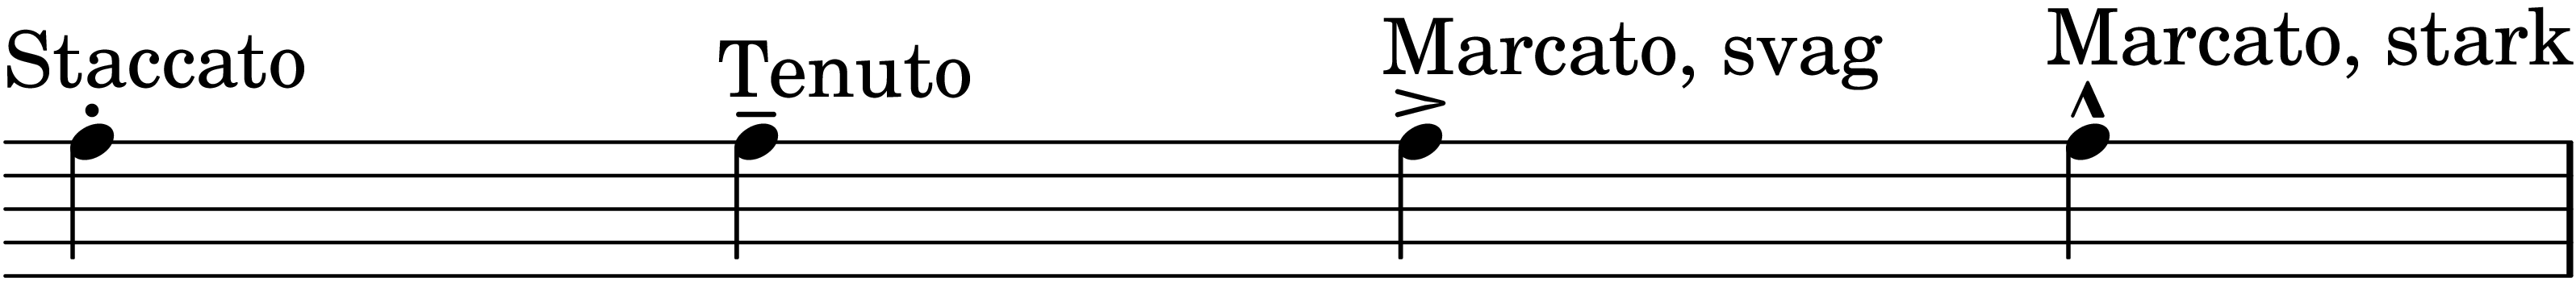
\includegraphics{lilypond/accents.cropped.png}
\end{center}

\textit{Staccato} innebär att tonen ska spelas kortare än det utskrivna notvärdet.

\textit{Tenutomarkeringen} signalerar att det är viktigt att tonen spelas med hela notvärdet. 

\textit{Marcato} innebär att tonen ska spelas starkare och mer markerat än övriga noter.

Det absolut tydligaste exemplet på när accenter är användbara är när en takt ska spelas staccato och noteras med korta notvärden och många pauser:

\begin{center}
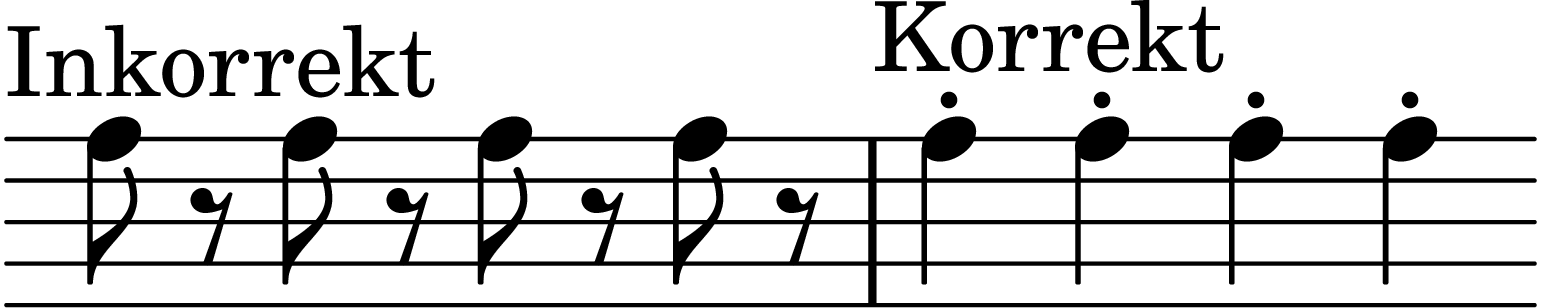
\includegraphics{lilypond/staccato.cropped.png}
\end{center}

Textmarkeringar kan ses på som den sista utvägen när varken dynamikmarkeringar, accenter eller andra notationsverktyg inte räcker till. Det är bra att sträva efter att musiker från hela världen ska kunna läsa ens arr, och då bör man förstås undvika att skriva kommentarer ovanför systemen. Det som kan accepteras är de vanliga (ofta italienska) tempo- och stilmarkeringarna och vissa teknikförslag som ibland anges i t.ex. kompmusikernas stämmor. 


\newpage
\vspace{2em}
\noindent\fbox{%
    \parbox{\textwidth}{%
        \section{Felstavad tonhöjd}
        Arrangerar man någonting krångligare än ``Blinka lilla stjärna'' stöter man så småningom på icke-diatoniska toner, det vill säga toner som inte egentligen tillhör tonarten låten går i. De flesta sådana toner går att skriva på två olika sätt, vilket kallas hur man stavar tonen. Exempelvis kan tonen mellan F och G skrivas som både F$\sharp$ och G$\flat$. 

        Vilket sätt man ska stava en ton är sällan fritt fram att välja själv, utan bestäms huvudsakligen av två saker. Den första är de omgivande tonerna. Betrakta nedanstående exempel av den första takten i Für Elise, och se vilken som verkar lättast att läsa:


\begin{center}
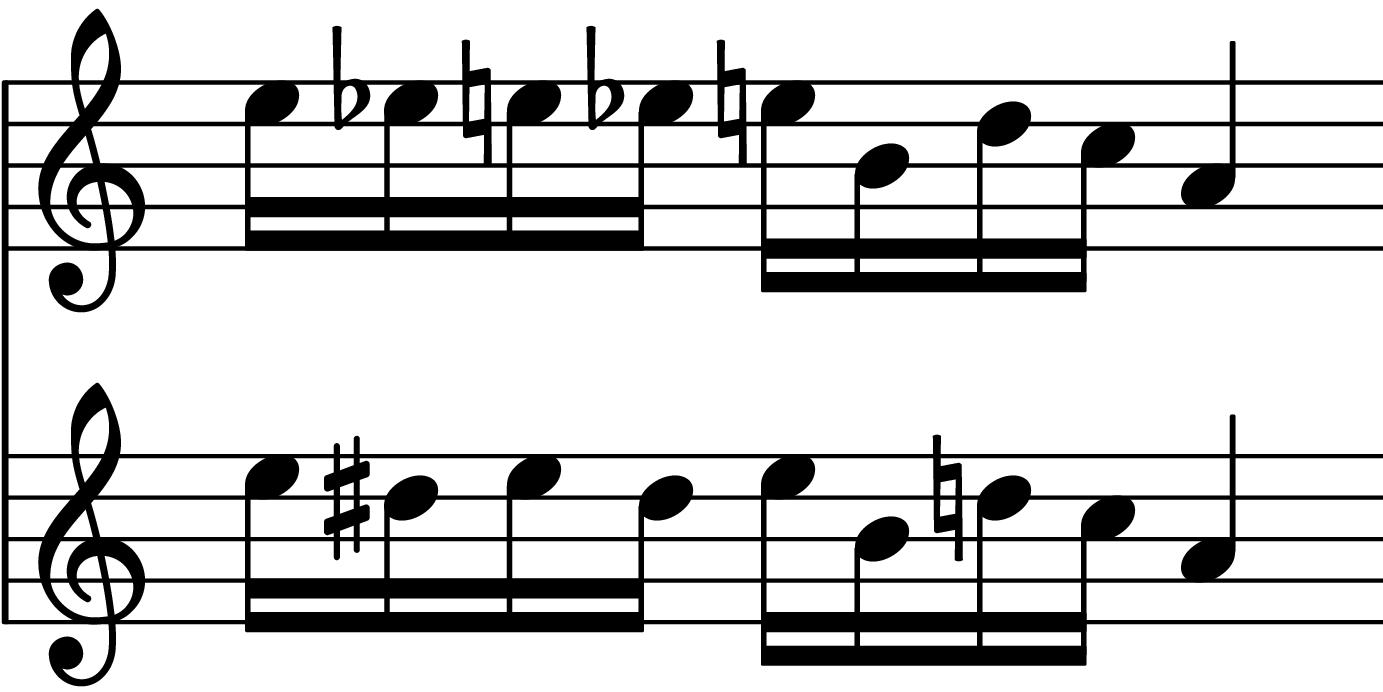
\includegraphics{lilypond/spelling-elise.cropped.png}
\end{center}

    Den nedre är betydligt lättare för en musiker att läsa, och i regel vill man helt enkelt minimera mängden tillfälliga förtecken på rad efter varandra. 

    Det andra som påverkar stavningen är ackordtoner. Om orkestern spelar ett D-dur-ackord så ska ingen spela G$\flat$, utan alla som spelar den tonen måste stava den F$\sharp$. Det finns ett fåtal undantagsfall som kan dyka upp i samband med transponerande instrument, men i allmänhet gäller regeln oavsett transponering.

    \vspace{1em}
        \textbf{Musescore}

        I Musescore finns ett verktyg för att automatiskt stava noter enligt det sätt som beskrivs ovan. Verktyget heter \textit{Respell pitches} och finns i kategorin \textit{Tools} i menyraden. På svenska heter samma verktyg \textit{Stava om tonhöjd} och finns i kategorin \textit{Verktyg}. Markera de takter som ska rättas till innan du startar verktyget, eller avmarkera taktmarkeringen för att korrigera alla takter i stycket.
    }%
}
